\section{Evaluation}\label{sec:evaluation}

Here we present our evaluation of the SEU protection approach. We first introduce three test applications with different degrees of stack dynamism. We then validate the correctness of our approach and analyze the relationship between protection efficacy and the SEU injection rate. Finally, we consider the overhead introduced by our approach, both in terms of space and execution speed. Ubuntu 13.10, with Linux kernel version 3.8, and GCC 4.1.2 are used.

\subsection{Test Applications}

To evaluate our approach under varying stack conditions and SEU injection rates, three AVR applications are considered. The stack usage pattern of each application is shown in Figure \ref{fig:stacksize_usage}. The x-axis represents execution time, and the y-axis represents stack size. Below is a description of each application.

\begin{itemize}
\item The \textbf{Delay} application repeatedly executes a function that contains a delay of 2,040 clock cycles, implemented using a while loop, yielding low stack variability.
\item The \textbf{Double Function Calls} application repeatedly executes three functions --- function A calls B, and function B calls C --- yielding moderate stack variability.
\item The \textbf{Fibonacci} application repeatedly calculates the tenth Fibonacci number using recursion, yielding significant stack variability.
\end{itemize}

\begin{figure}[h]
\centering
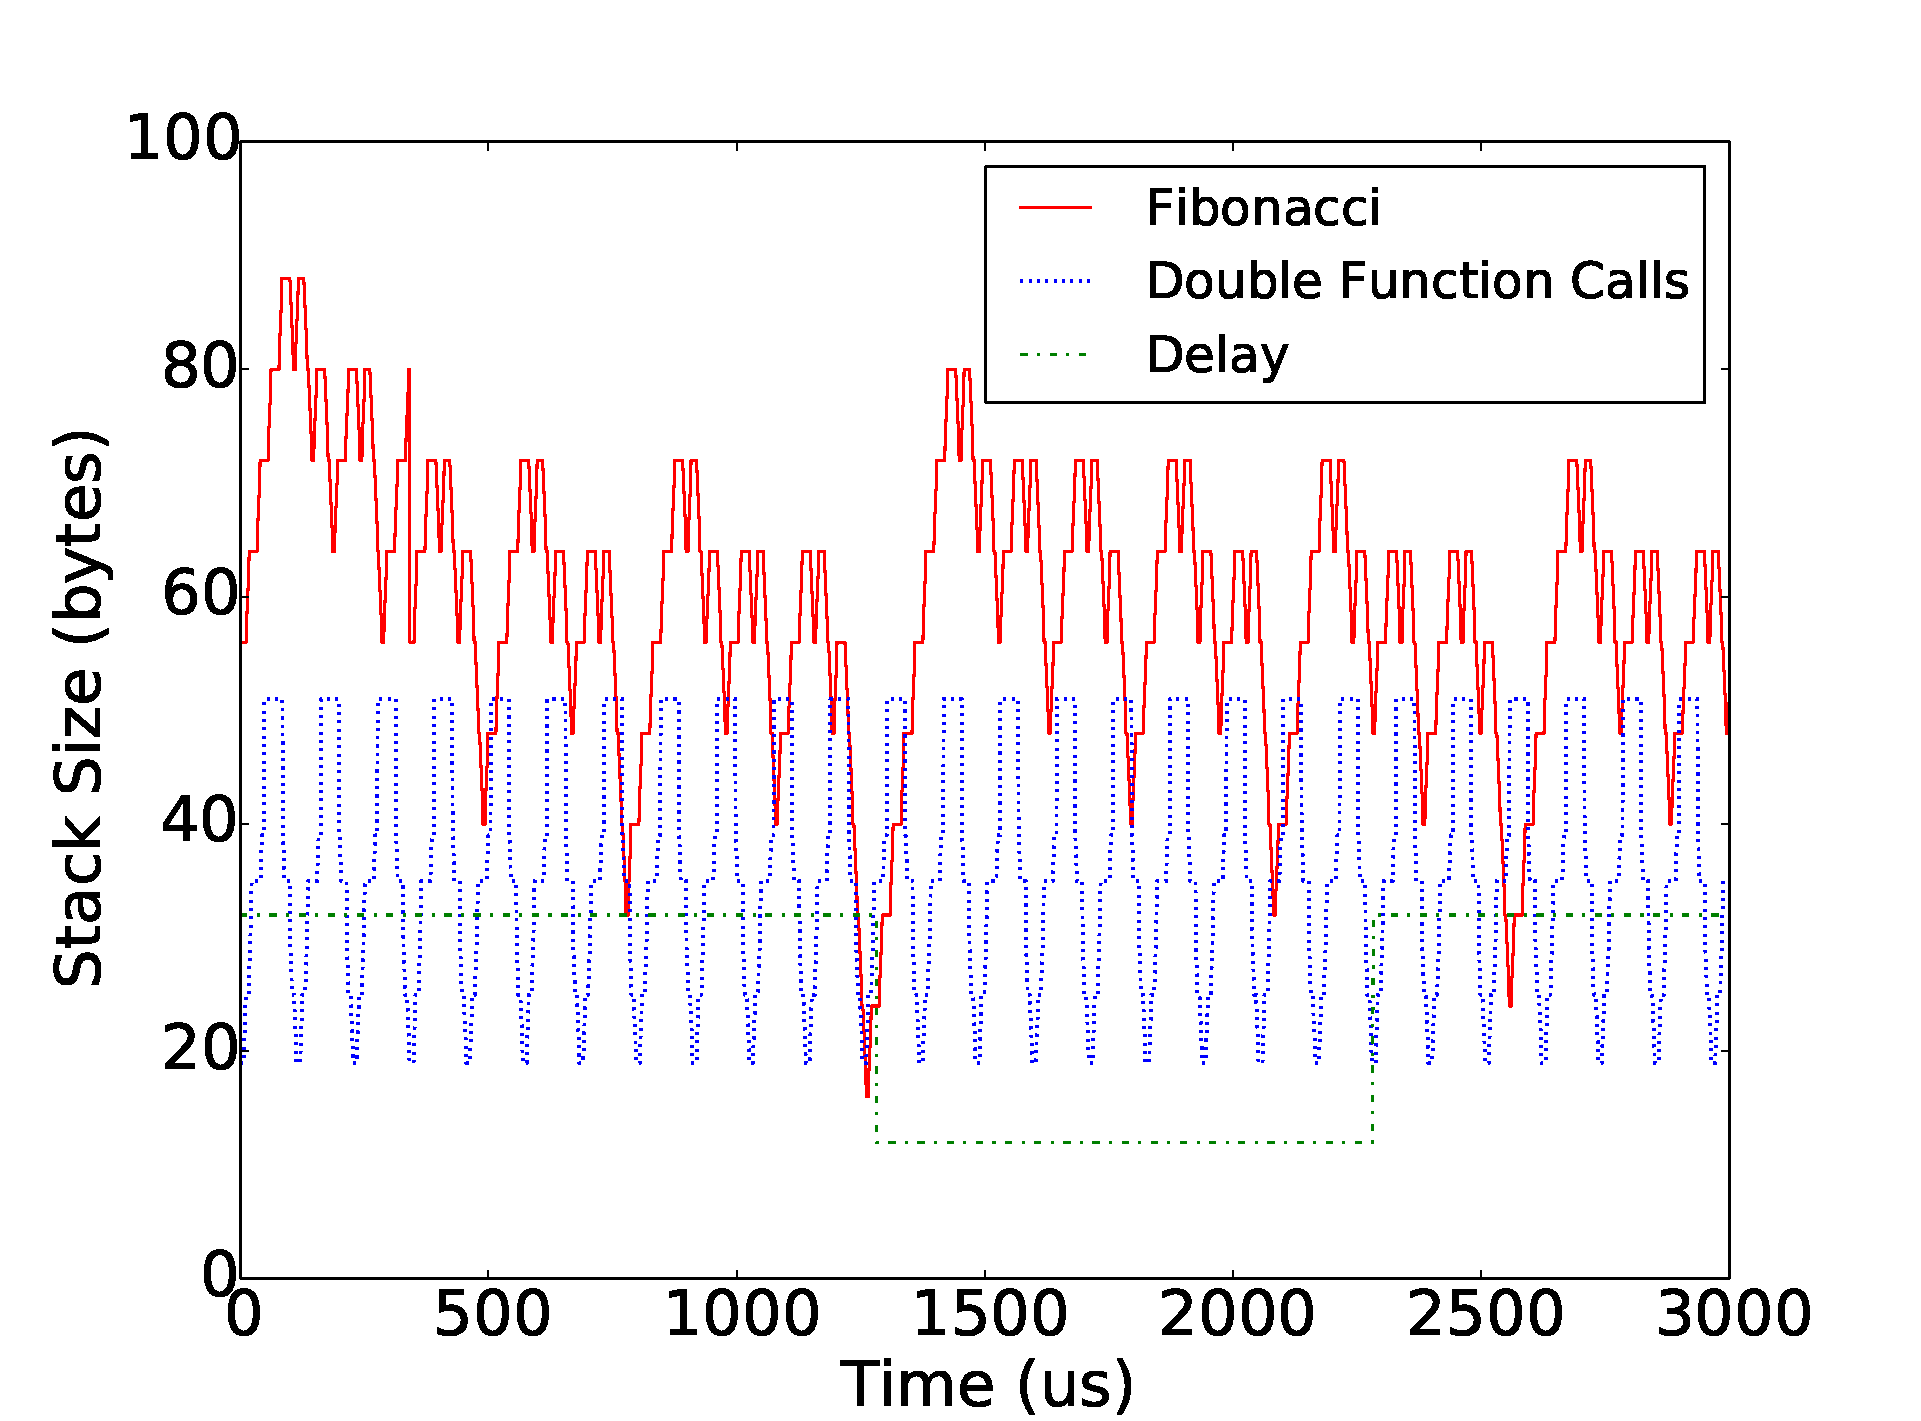
\includegraphics[width=0.48\textwidth]{figures/stacksize_usage_v3.pdf}
\vspace{5pt}
\caption{Stack Usage of Test Applications}
\label{fig:stacksize_usage}
\end{figure}

\subsection{Validation}

We first validate our approach and consider the SEU protection efficacy it affords. Recall the modified SRAM partition shown in Figure \ref{fig:modified_ram_map}. In our analysis, we ignore both the .data and the .bss sections, as well as the heap section. Data stored in the .data, .bss, and heap sections can be protected using well-known techniques based on cloning and comparison. We focus our analysis on stack frame protection. Again, the injected code segments used to protect the stack frames are designed to use only registers, and each segment requires only two bytes in the currently executing function's stack frame (for the return address).
%A embedded application is typically designed based on interrupts, and usually contains an infinite loop in a function, which never returns. If the function which has the infinite loop is not the \textit{main} function (although it is the \textit{main} function for most times), the stack frame of the function's caller is not protected. However, since the stack space containing the function and its callers' stack frames doesn't change during the execution of the applications, the space can be identified using static analysis and can be protected using cloning and comparison. This issue will be addressed in our future work.

We first assume that the currently executing function's frame, which includes the return address of the injected code segment, is not affected by SEUs. We use induction to prove the correctness of our approach. Suppose \textit{n} is the number of stack frames stored in the stack, excluding the frame for \textit{main}.

\textbf{Base Case:} If $n=0$, only the stack frame of \textit{main} is on the stack. When \textit{main} calls another function, say \textit{foo}, the stack frame for \textit{foo} is created. According to our assumption, the current stack frame (\textit{foo}'s) will not be affected by SEUs during execution. When \textit{foo} returns, the stack frame of \textit{main} is protected by our approach. So the stack frames of caller and callee are guaranteed to be correct if any function is invoked and returns when $n=0$.

\textbf{Induction Assumption:} Assume that the stack frames of callers and callees are guaranteed to be correct for $n=k$, where $k\geq 1$.

\textbf{Inductive Step:} Now consider $n=k+1$. Assume \textit{a} is the current function, which calls \textit{b}. According to our assumption, b's stack frame is not affected by SEUs. When \textit{b} returns, the stack frame of \textit{a} is protected by our approach. So the stack frames of callers and callees are guaranteed to be correct when $n=k+1$. The currently executing function's stack frame is assumed safe, and the stack frames of callers and callees are protected against SEUs during execution; by induction, the stack is guaranteed to be correct, assuming the current stack frame is never affected by SEUs.

To verify this claim, the AVR Simulator IDE~\cite{avrsimide} was used to manually inject SEUs, and to observe execution results. The results showed that each function is able to detect and fix SEUs introduced ``beneath'' the topmost stack frame.

However, if the stack frame of the current function is affected by an SEU, protection is not guaranteed. If the SEU changes key data, such as the return address or stack frame size, the current function will not execute as expected. We assume that only one SEU will occur during a given function execution, and that the SEU is uniformly likely to affect all bits in RAM. The probability of successful SEU protection can be expressed as:
\begin{equation}\label{eq_seu1}
p=1-\frac{c}{2s+e-c+6}
\end{equation}
Where $p$ is the probability of successful protection, $s$ is the stack size, $e$ is the size of the unused space in RAM, $6$ is the size of the three STP copies, and $c$ is the average size of a stack frame. Since the return address of the injected code segment is stored in the current stack frame, the two bytes for the return address are included in c. The total size of protected memory is $s+e+(s-c)+6$, where $s-c$ is the size of the stack frame copies stored in the \textit{md} section.

We extend our analysis to cases where more than one SEU may occur during a given function execution. Our approach succeeds when the following conditions are met: (i) the currently executing function's stack frame is not affected (so the return address of the injected code segment is not affected); (ii) at least two of the three copies of the caller's stack frame size are not affected; (iii) at least two of the three copies of the STPs are not affected; and (iv) at least one of the two caller's stack frames (the original and the backup copy saved in the \texttt{md} section) is not affected. To simplify the analysis, conditions (ii) and (iii) are strengthened, requiring that all three copies of the caller's stack frame size cannot be affected, and all three copies of the STPs cannot be affected. Since the strengthened conditions slightly reduce the probability of successful SEU protection (only 4 bytes are ignored), the real probability of protection is slightly higher than the presented results. The probability of successful SEU protection can be expressed as:
\begin{equation}\label{eq_seu2}
\begin{split}
&p=(1-\frac{c}{2s+e-c+6})^n*(1-\frac{6}{2s+e-2c+6})^n \\
&*(1-\frac{6}{2s+e-2c})^n*\{(1-\frac{2c}{2s+e-2c-6})^n \\
&+ \mathrm{C}_2^1*(1-\frac{c}{2s+e-2c-6})^n\\
&*[1-(1-\frac{c}{2s+e-3c-6})^n]\}
\end{split}
\end{equation}

Where $p$ is the probability of success, $s$ is the size of the stack, $e$ is the size of the unused space in RAM, $6$ is the size of the three stack frame size copies or the three STP copies, $c$ is the average size of the stack frame (including the return address of the injected code segment), and $n$ is the number of SEUs that occur during a function's execution. In equation \ref{eq_seu2}, $(1-\frac{c}{2s+e-c+6})^n$ is the probability that the currently executing function's stack frame is not affected by SEUs. $(1-\frac{6}{2s+e-2c+6})^n*(1-\frac{6}{2s+e-2c})^n$ is the probability that both copies of the caller's stack frame size and the three STPs are not affected by SEUs. Within the curly brackets, $(1-\frac{2c}{2s+e-2c-6})^n$ is the probability that both the original and the copy of the caller's stack frame are not affected by SEUs. $\mathrm{C}_2^1*(1-\frac{c}{2s+e-2c-6})^n*[1-(1-\frac{c}{2s+e-3c-6})^n]$ is the probability that either the original or the copy of the caller's stack frame is affected by SEUs. So $\{(1-\frac{2c}{2s+e-2c-6})^n + \mathrm{C}_2^1*(1-\frac{c}{2s+e-2c-6})^n*[1-(1-\frac{c}{2s+e-3c-6})^n]\}$ is the probability that at least one --- the original or the copy --- of the caller's stack frames is not affected.

In equation \ref{eq_seu2}, the number of SEUs that occur, $n$, can be expressed as:
\begin{equation}
n = \frac{y*l}{m}*f
\end{equation}
where $y$ is the number of clock cycles used to execute each instruction, $m$ is the frequency of the microprocessor, $l$ is the average number of function instructions, and $f$ is the SEU injection rate. Most AVR instructions require 2 clock cycles to execute, and the frequency of our ATmega644 is set to 10MHz.

\begin{table}
	\center
    \begin{tabular}{|l|c|c|c|c|}
    \hline
    \textbf{Applications}   & \textbf{l} & \textbf{c} & \textbf{s} & \textbf{e}	\\ \hline
    Fibonacci             		& 42			& 10		& 60	   	& 2992		\\
\hline
    Double Function Calls       & 54			& 9			& 30        & 3022		\\ \hline
    Delay         				& 115			& 16		& 30		& 3022		\\
 \hline
    \end{tabular}
    \vspace{5pt}
    \caption {Application Characteristics}
    \label{tbl_application_parameters}
\end{table}
\begin{figure}
\centering
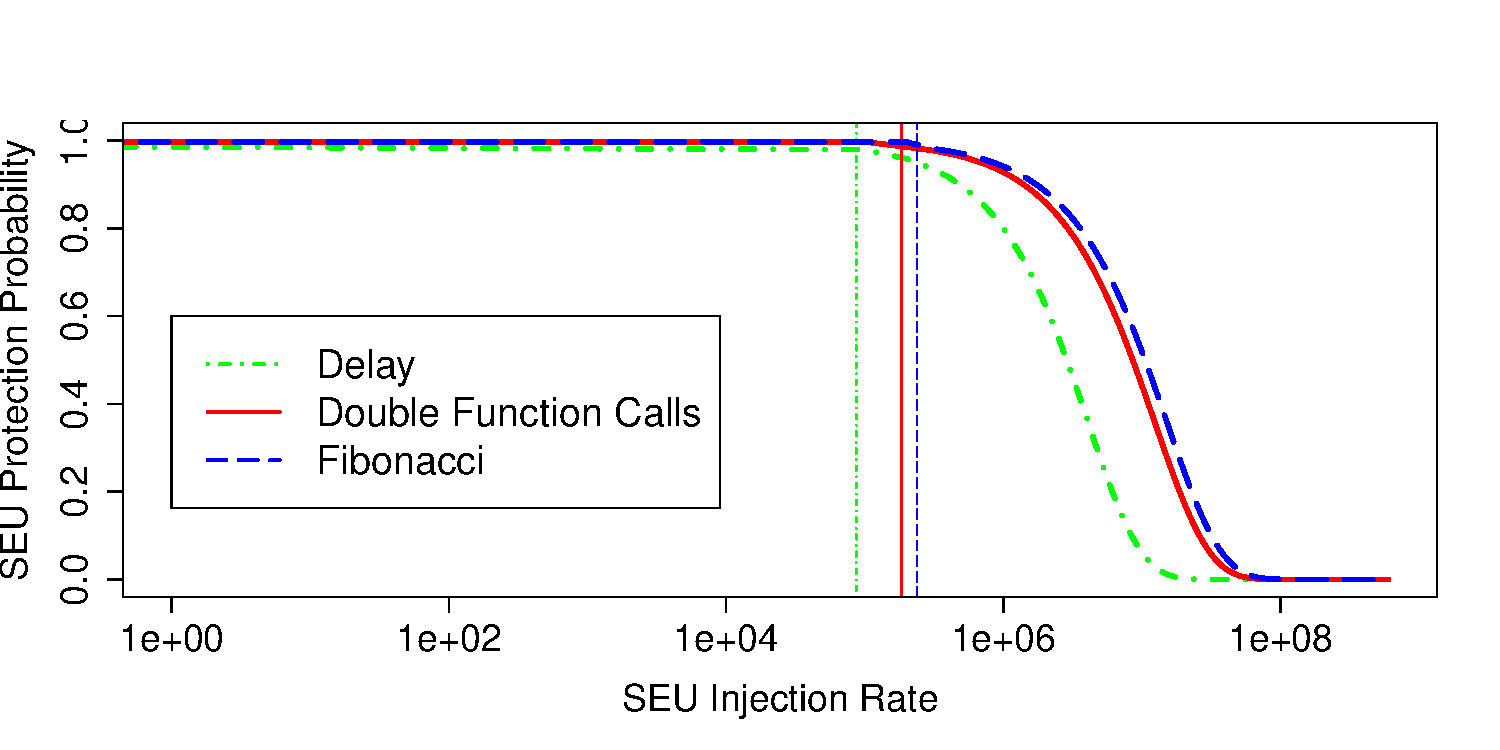
\includegraphics[width=0.48\textwidth, height=130pt]{figures/success_probability_v2.pdf}
\vspace{5pt}
\caption{SEU Protection Probability}
\label{fig:success_probability}
\end{figure}
We now consider the relationship between SEU protection probability and SEU occurrence rate. To demonstrate the relationship, we collect the corresponding parameters for the three test applications using AVR Simulator IDE, as shown in Table \ref{tbl_application_parameters}. Figure \ref{fig:success_probability} plots the change in SEU protection probability as a function of SEU injection rate. The x-axis represents the rate at which SEUs are injected, and the y-axis represents the corresponding SEU protection probability. Each vertical line marks where the number of SEUs begins to exceed 1 (for each application). When only one SEU occurs during a given function execution (left side of the vertical line), the SEU protection probability is constant (Delay: 99.48\%, Double Function Calls: 99.71\%, Fibonacci: 99.68\%) because the only case the approach cannot handle is when the current frame is affected. When more than one SEU occurs during a given function execution (right side of the vertical line), the SEU protection probability increases because the SEUs may affect the stack frame of the current function, the stack frame sizes of the caller stored in the stack, the STPs, and stack frame copies stored in the \texttt{md} section. As the SEU occurrence rate increases, the SEU protection probability decreases, until it approaches 0. The lower the stack dynamism, the longer the function execution time, which increases the probability of SEU occurrence in the current stack frame. Low stack frame dynamism causes the SEU protection probability for Delay to drop significantly compared to the other applications.

\subsection{Performance}

Since the same code is injected for every function, the execution overhead is similar for all functions, varying only when an SEU is detected. Table \ref{tbl_speed_overhead} summarizes the overhead of each injected code segment. The second column lists the number of times each code segment executes (per function execution), the third column lists the number of instructions executed in each code segment, the fourth column lists the number of clock cycles spent executing each code segment, and the fifth column lists the ROM space overhead for each injected segment. $S$ denotes the size of the (recovered) stack frame. The \textit{CRC calculation} code segment and \textit{STP update} code segment execute twice for each function, and the \textit{frame copy} code segment executes either once or twice, depending on whether an SEU is detected. Each of the other code segments executes once for each function execution. Therefore, the minimum overhead introduced in terms of number of clock cycles is $62*S+304$, when an SEU is not detected. The worst case is $70*S+432$ clock cycles, when an SEU is detected. 
\begin{table*}
	\center
    \begin{tabular}{|l|c|c|c|c|}
    \hline
   \textbf{Code Segment}   & \textbf{Number of Execution} & \textbf{Instructions} & \textbf{Clock Cycles} & \textbf{ROM Space}	\\ \hline
    CRC Calculation         & 2			& 24*S+1		& 27*S+4		& 50				\\ \hline
    CRC Save                & 1			& 13			& 26           	& 26				\\ \hline
    CRC Compare             & 1			& 27			& 52		   	& 64				\\ \hline
    Frame Copy				& 1 or 2	& 64+4*S		& 8*S+128      	& 50				\\ \hline
%    Frame Copy (Worst Case) & 1 		& 73+4*S      & 144+8*S      & 50				\\ \hline
    Frame Size save         & 1			& 18			& 34           	& 36				\\ \hline
    STP Initialization		& 1			& 16			& 28		   	& 32				\\ \hline
	STP Update				& 2			& 7				& 14			& 14				\\ \hline
	\textbf{Total (No Recovery)} & -	 	& 48*S+154     	& 62*S+304		& 272  		\\ \hline
	\textbf{Total (Recovery)}& -	 		& 52*S+218     	& 70*S+432		& 272 		\\ \hline
    \end{tabular}
	\vspace{5pt}
    \caption {Execution Overhead}
    \label{tbl_speed_overhead}
\end{table*}

We next evaluate space overhead using the three test applications. The ROM space data was collected using \textit{avr-size}. The results are summarized in Figure \ref{fig:space_overhead}. The y-axis represents ROM size, in bytes. Delay and Fibonacci involve two functions, and Double Function Calls involves four. From Figure \ref{fig:space_overhead}, we can see that the ROM overhead for the Double Function Calls application is twice the Delay and Fibonacci applications. ROM overhead is related only to the number of functions in the program.

\begin{figure}[h]
\centering
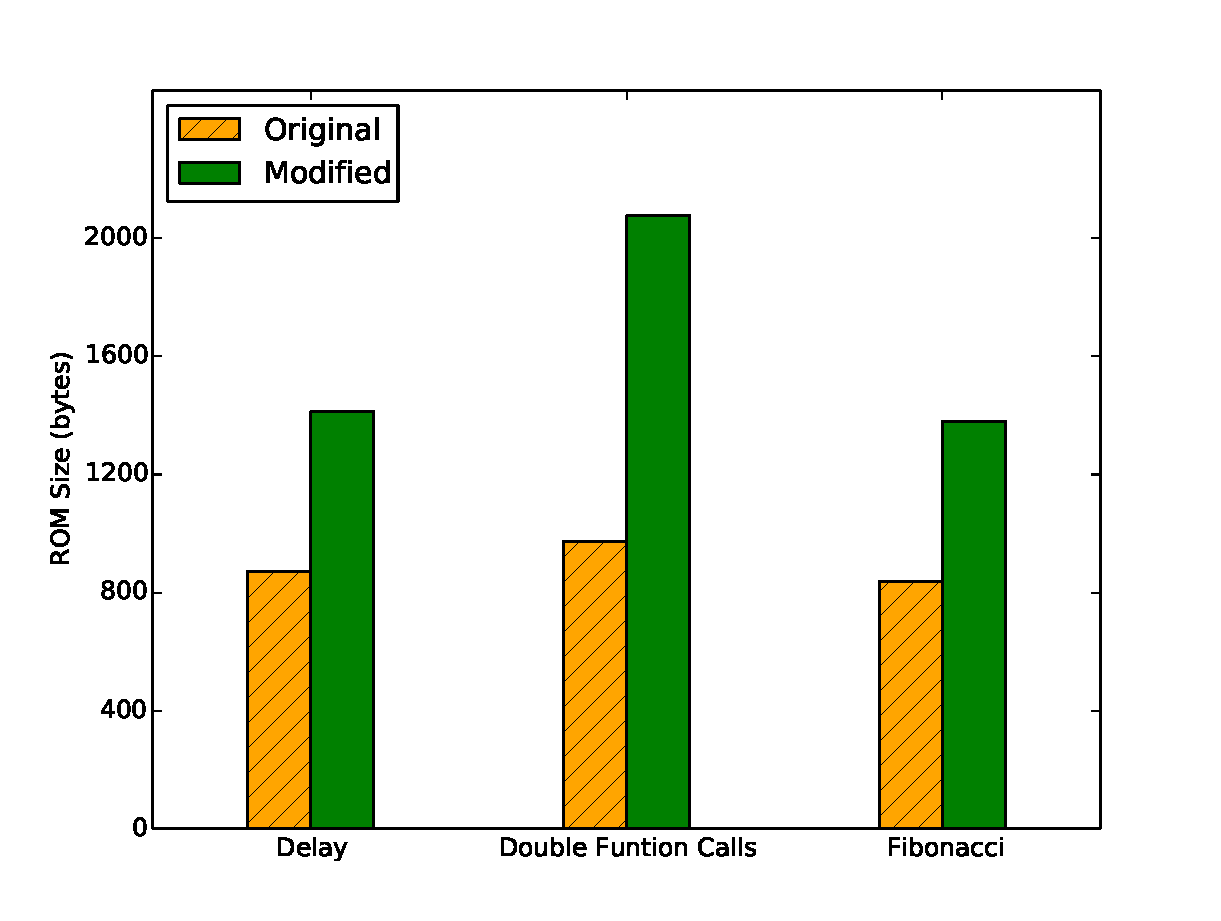
\includegraphics[scale=0.47]{figures/space_overhead.pdf}
\caption{ROM Overhead}
\vspace{5pt}
\label{fig:space_overhead}
\end{figure}

We next evaluate execution overhead. As shown in Table \ref{tbl_speed_overhead}, the execution overhead for every function call is determined by the size of the stack frame. We consider the execution overhead as a function of the average number of instructions executed between each call instruction (i.e., an inverse measure of call frequency). The execution overhead can be expressed as:
\begin{equation}\label{eq_seu1}
e=\frac{l+L}{l}
\end{equation}
Where \textit{L} is the number of injected machine instructions for each function, and \textit{l} is the average number of machine instructions executed between each call instruction. As summarized in Table \ref{tbl_speed_overhead}, $L=48*S+154$ when no SEUs are detected, and $L=52*S+218$ when an SEU is detected. The average frame size, $S$, is 20. The overhead results are summarized in Figure \ref{fig:speed_overhead}. The x-axis represents the average number of instructions executed between function invocations (\textit{l}), and the y-axis represents execution overhead, measured as the ratio between the execution speed of the original code and the modified code. The figure shows that given the same stack frame size, execution overhead is determined by stack dynamism. The less stack dynamism, the less speed overhead. The explanation is that within a given period of time, increased function calls lead to increased execution of the injected code. The results reveal an interesting tradeoff among dynamism, protection efficacy, and performance. Increasing dynamism offers better protection, but worse performance; decreasing dynamism offers better performance, but less protection. Knowledge of this tradeoff can be used to inform the function decomposition process, enabling embedded designers to appropriately balance protection efficacy and execution overhead.
\begin{figure}
\centering
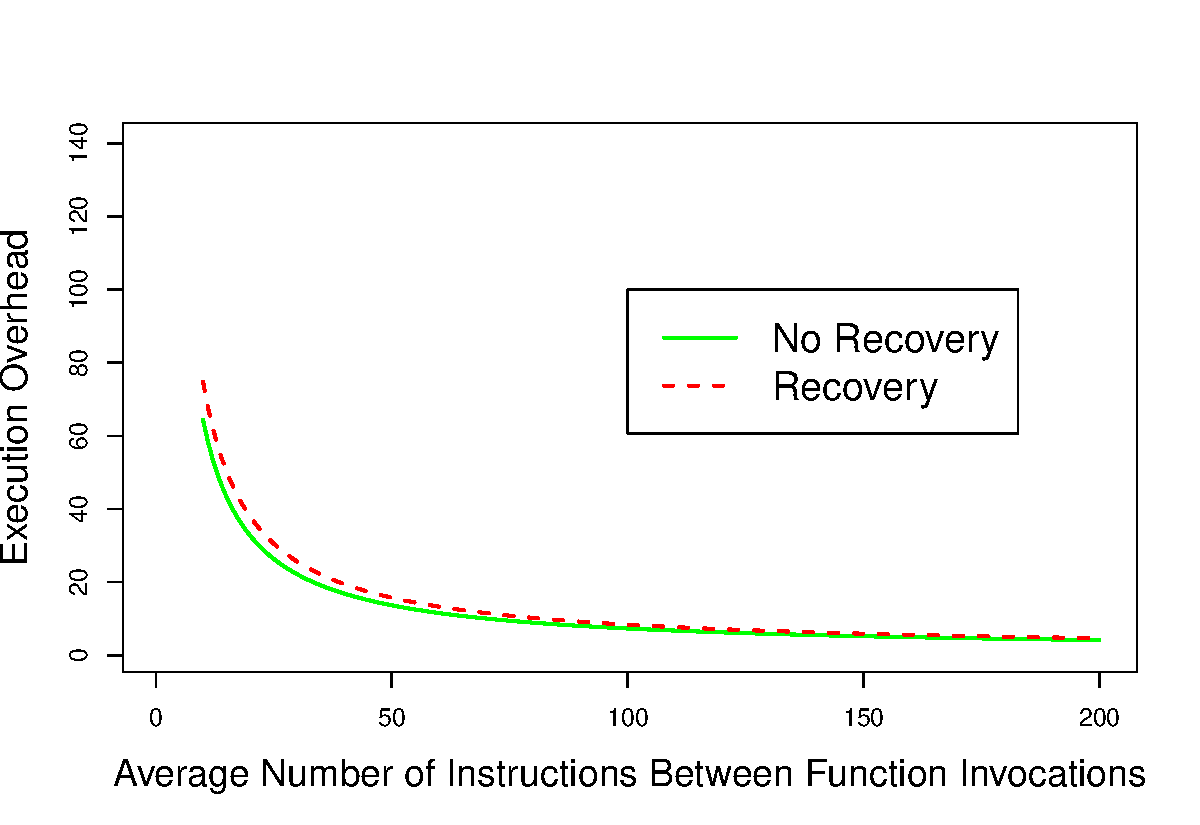
\includegraphics[width=0.47\textwidth]{figures/speed_overhead_line_chart_v1.pdf}
\vspace{5pt}
\caption{Execution Overhead}
\label{fig:speed_overhead}
\end{figure}

\subsection{Progressive Test}
In verifying our approach on physical hardware, we emulate the occurrence of SEUs by flipping random bits in the target SRAM area. To perform auditable test runs, we developed an AVR application which continuously generates an increasing integer sequence, which is then sent to the UART interface at a controllable speed. A Python program running on a desktop is used to receive the sequence and observe the impact of flipped bits by monitoring the continuity of the sequence. A timer interrupt is used to trigger the occurrence of SEUs. The interrupt service routine function generates a random address within the range of the top of the stack and the end of RAM space, excluding the stack frame of the current interrupt, and then flips the bit at this location. The bit flip frequencies are set to $10^7$Hz, $1.25*10^6$Hz, $1.5625*10^5$Hz, $39062.5$Hz, and $9765.625$Hz.\footnote{These frequencies are derived from the built-in timer prescaler of the Atmega644, at 1, 8, 64, 256, and 1024, respectively}. An Atmega644 microprocessor is used in our experiments.

We declare (observable) failure when one of the following two situations occurs: (i) The AVR application stops generating integers; or (ii) the integer sequence received by the Python program becomes discontinuous. We monitor the integer sequence and record the maximum count before failure. The experimental results are summarized in Figure \ref{fig:exp1_result}. The x-axis represents the SEU injection frequency, and the y-axis represents the maximum count received by the Python program. The figure shows that as the SEU injection frequency increases, running time to failure decreases. This is explained as follows: As the SEU injection frequency increases, the probability that an SEU occurs in a critical area increases. When the frequency is extremely high (e.g. approximate 10 MHz), the program can hardly send any values. However, the observed SEU occurrence rate in outer space is approximate $10^{-6}SEU/bit$-$Day$~\cite{underwood1992observations}. Given the total RAM size of Atmega644 is 4K Bytes, the SEU occurrence rate of Atmega644 is 0.0032 SEU/day, which is significantly lower than the lowest frequency (9765.625 SEU/second) that we used. So this situation will be extremely rare in a realistic scenario.

%We declare (observable) failure when one of the following two situations occurs: (i) The AVR application stops generating the integers; or (ii) the integer sequence received by the Python program becomes noncontinuous. We monitor the integer sequence and record the maximum count before failure. In the experiment, the Atmega644 microprocessor runs at $10^7$Hz. The error insertion frequencies are set to $10^7$Hz, $1.25*10^6$Hz, $1.5625*10^5$Hz, $39062.5$Hz, $9765.625$Hz.\footnote{derived from the built-in timer prescaler of Atmega644, at 1, 8, 64, 256, 1024, respectively} The \textit{delay} function is used to control integer sequence generation frequency, which is set to 1Hz, 10Hz, 100Hz, and 1000Hz. The experimental results are summarized in Figure \ref{fig:exp1_result}. The x-axis represents the error insertion frequency, and the y-axis represents the maximum count received by the Python program. The figure shows that given the same error insertion frequency, as the program running speed increases, the maximum integer received by the Python program increases. This is because that since the probability of SEUs occur on critical area is fixed, faster program running speed will generate more numbers. Given the same integer generation frequency, as the error insertion frequency increases, the maximum correct number received by the Python program decreases. This is explained as follows: as the error insertion frequency increases, the probability that SEUs occur on critical area increases. When the error insertion frequency is extremely high, the program can hardly send anything. However, the observed SEU occurrence rate is approximate $10^{-6}SEU/bit$-$Day$ in the outer space~\cite{underwood1992observations}, which is significantly lower than our test frequencies.

\begin{figure}
\centering
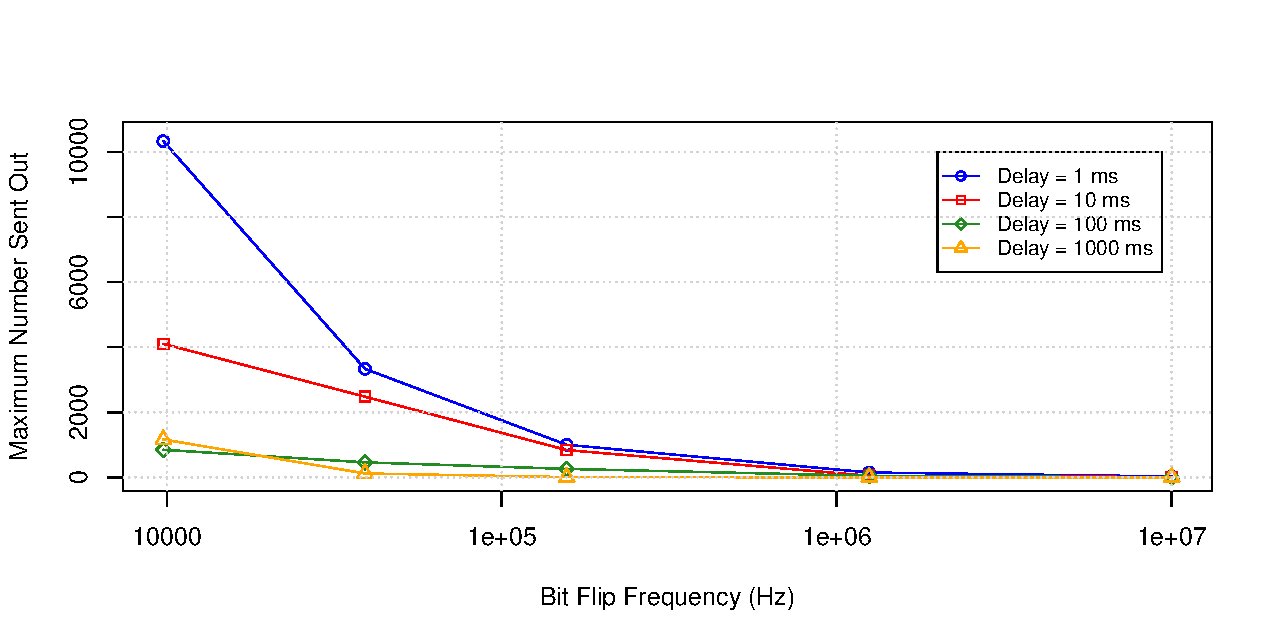
\includegraphics[scale=0.4]{figures/experiment1.pdf}
\caption{SEU Experiment Results}
\vspace{5pt}
\label{fig:exp1_result}
\end{figure}



